\section{An I/O Efficient Vertex-Centric Storage Method for Property Graph}\label{sec:storage}
The random access problem is a well known hard problem for out-of-core systems,
especially for the graph related problem, which is notorious for its poor locality~\cite{DBLP:conf/osdi/KyrolaBG12}.
The traditional way to store graphs on disk is the double list method:
Stores the in-edges and out-edges separately for each vertex,
via the compressed sparse column (CSC) and the compressed sparse row (CSR) format~\cite{DBLP:conf/sc/PearceGA10}.
However, we find that this storage method have limitations to solve the real-world property graph matching problem:
\emph{Random disk accesses are unavoidable when in/out-edges are stored separately}.

To solve the random disk access problem, in this section,
we propose a novel property graph storage engine from a vertex-centric point of view.
Noticeably, only part of the huge billion node data graph would be read when solving a property graph matching problem,
with the help of a few easy to implement indices.
And all the disk reads are sequential.
Moreover, by using the property graph matching engine that will be discussed in the next section,
we would be sure that the huge data graph would be read at most once.
\subsection{Scan the Data Graph Sequentially}
The property graph matching problem requires the complete connection information between vertices,
however, the conventional double list storage method break up the completeness and results in random disk accesses.

Consider the patten graph in Figure~\ref{img:celebrity_star}, which simply finds friendship pairs in a data graph.
If two vertices in the data graph, say $v_i$ and $v_j$, are supposed to match the pattern,
we must be sure that $v_i$ and $v_j$ follows each other at the same time.
This kind of neighbor checking is also the most essentially building block of a property graph matching engine.

In the data graph, $v_1$ has $m$ in-edges and $n$ out-edges, and suppose that they are stored separately in the traditional way.
In order to determine whether $v_1$ could match $u_1$,
one has to scan the in-edges (or equally, the out-edges) of $v_1$ and then check whether the visited neighbor is in the out-edges (or in-edges) list.
This scan and check method would significantly slow down the graph matching process,
because the checking process results in random disk read.
For real world power-law graphs, where the celebrities or trending topics have a huge amount of followers,
the in/out-edges lists stored on disk have to be swapped in and out frequently during the scan and check process as a result of the random disk access pattern.
And it would be more complicated if there are more than two edges between $u_1$ and $u_2$ in the pattern graph.
\begin{figure}[ht]
  \centering
  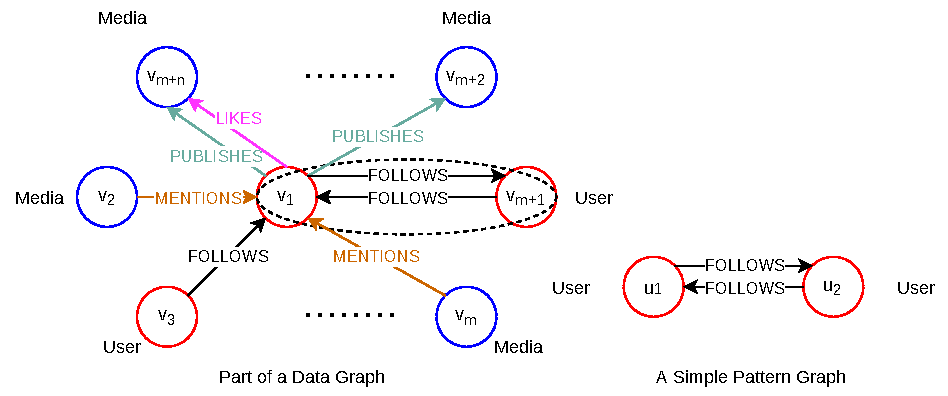
\includegraphics[width=0.38\textwidth]{img/celebrity_star.pdf}
  \caption{A celebrity with a huge amount of followers and a pattern graph to find friendship pairs in it.}\label{img:celebrity_star}
\end{figure}

The source of the problem is that the in/out-edges are stored separately in the conventional method,
whereas the property matching process need to retrieve both in- and out- connection information to determine whether a neighbor vertex could be matched.
Based on this observation, we propose a vertex-centric property graph storage method that always keeps the necessary connection information together for graph matching.
Take Figure~\ref{img:data_neighbors} as an example, which shows the logical storage structure for the celebrity in Figure~\ref{img:celebrity_star}.
Real-world property graphs are directed labeled graphs, instead of splitting the edges into in/out-edges,
we treat all the neighbors equally and store the connection information together with the neighbor vertex.
The specific edge information (direction, types) could be obtained by the position of the stored edge labels, i.e.,
the upper labels means the direction is pointed to the root and the lower labels means the opposite.
For example, the ``:FOLLOWS'' at the upper right corner of $v_3$ means $v_3$ follows $v_1$,
the two ``:FOLLOWS'' besides $v_{m+1}$ indicate that $v_1$ and $v_{m+1}$ follow each other.
And multiple edges are ubiquitous in property graphs, we support that by store the edge labels in a sequence,
as is shown in the figure where $v_1$ publishes a social media $v_{m+n}$ and also likes it.

By storing the neighbors in our vertex-centric approach,
all the necessary information are now stored locally together with the vertices,
and the neighborhood checking process of a property graph matching engine could be accomplished efficiently within a sequential disk scan.
For the pattern in Figure~\ref{img:celebrity_star}, if we suppose that $v_1$ matches $u_1$ and want to check whether the neighbors of $v_1$ would match $u_2$, we could just scan the neighbors and check the labels sequentially and find that $v_{m+1}$ would match.
No random disk access appears during the whole process, and there is no need to use complex indices to check the edge labels.
\subsection{Simple Indices to Reduce I/Os}
Despite of the fact that the size of the whole data graph could be gigantic,
we may only care a fraction of the graph by specify the labels in our query for a concrete graph matching problem.
There are two basic operations for a graph database to solve a graph matching problem:
1. Given a data vertex, retrieve the neighbors of it with a specific label;
2. Given a vertex label, retrieve the data vertices with the label.
In the following paragraphs, we'll show how to make the two operations efficiently by adding a few simple but efficient indices to the vertex-centric storage engine,
which reduces the searching space and I/O significantly.

Consider again the pattern graph in Figure~\ref{img:celebrity_star}, where we only care about the users in the social network,
no matter how much social media a user have published or viewed we could just ignore all of them in our specific problem.
A straightforward idea is to group the neighbor vertices with the same label together when storing the vertices.
However, if the neighbor vertices were stored in the traditional in/out-edge double lists method,
we have to group them twice and then still face the information insufficient problem as we discussed in the previous subsection.
As for our vertex-centric storage method,
the index could be added to the storage engine easily as is shown in Figure~\ref{img:data_neighbors},
where we simply store the key-value pairs that maps the vertex labels to the starting/ending position of the neighbors on disk.
Since it is used to locate only the neighbors of a specific vertex, we refer to this kind of index as \emph{local index}.
With the help of local index, we could skip all the useless neighbor vertices and only scan the necessary ones.
\begin{figure}[ht]
  \centering
  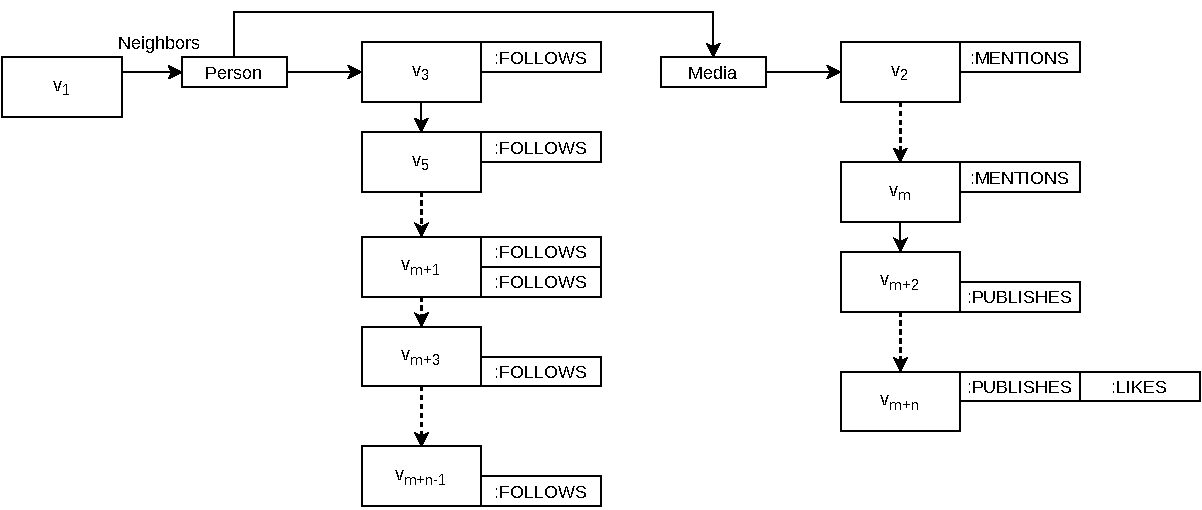
\includegraphics[width=0.48\textwidth]{img/data_neighbors.pdf}
  \caption{The vertex-centric storage structure of the celebrity $v_1$ in Figure~\ref{img:celebrity_star}.}\label{img:data_neighbors}
\end{figure}

From a higher perspective, in order to solve a property graph matching problem,
one need to firstly select a starting vertex in the data graph,
regardless of the concrete graph matching algorithm whether it is tree based or join based.
There is no need to scan all the vertices in a billion node data graph if we only care about vertices with the specific labels.
Just like the local index we discussed above, we could add a global index which contains key-value pairs that maps the labels to the corresponding position on disk (Figure~\ref{img:data_vertices}).

In summery, for a property graph matching problem, we could quickly jump to the domain of interest with the help of the global index, and then scan and check only the necessary neighbors with the help of our local index.
After jump to the correct position, all the disk reads are sequential.
\begin{figure}[ht]
  \centering
  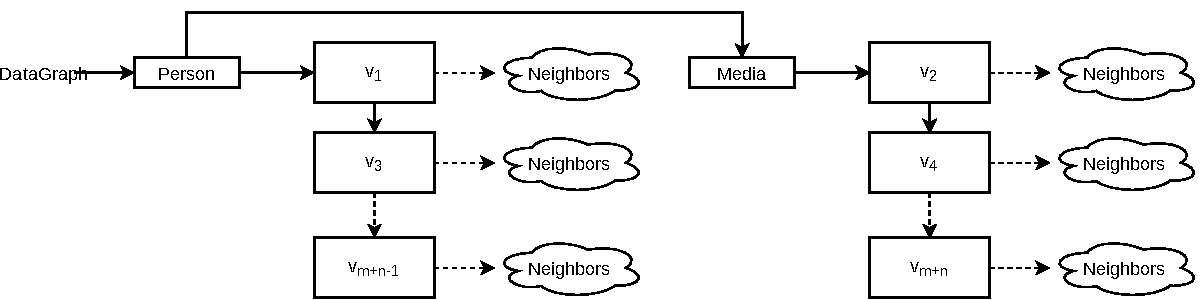
\includegraphics[width=0.48\textwidth]{img/data_vertices.pdf}
  \caption{The storage structure overview of the data graph in Figure~\ref{img:celebrity_star}.}\label{img:data_vertices}
\end{figure}
\subsection{Remarks on the Implementation of the Storage Method}
For applications that need to perform the two basic operations (visiting vertices and visiting the neighbors),
we define two iterators as the interface to visit the data graph:
\begin{enumerate}[noitemsep]
\item \textsc{VertexIter}: Given a vertex label, it iterates through the vertices with the specified label ordered by the ID of vertices;
\item \textsc{NeighborIter}: Given a data vertex and a label, it visits the neighbors with the label, the neighbors are also sorted by the IDs.
\end{enumerate}
In Section~\ref{sec:match} we'll show that the sorting constraint could boost the matching of property graphs.

These iterators could be implemented efficiently by using our vertex-centric storage model.
And we also provide a compact disk format implementing the vertex-centric storage model in Figure~\ref{img:data_graph}.
Vertices are sorted by their IDs, and we store in/out-degrees as early filters when scanning the vertices.
Edge labels are stored as integers here, however, bitmap could also be used for higher performance.
The \textsc{VertexIter} just searches the global index and then visits the disk data sequentially;
The \text{NeighborIter} scans the neighbors with the help of the local index.

Please note that the vertex-centric storage model is not restricted to this disk format.
In fact, as long as a storage engine could implement the two iterators efficiently,
it could implement the vertex-centric storage model well.
For example, the sorted vertices could be replaced with B-tree to make the insertion/deletion operation easier for dynamic graphs.
It is also possible to implement the vertex-centric storage model in memory as buffer cache for existing graph databases to achieve better locality.
Moreover, we are now working on implementing the vertex-centric storage model on top of relational database to embrace the power of the half-century-year-old mature technology.
\begin{figure}[ht]
  \centering
  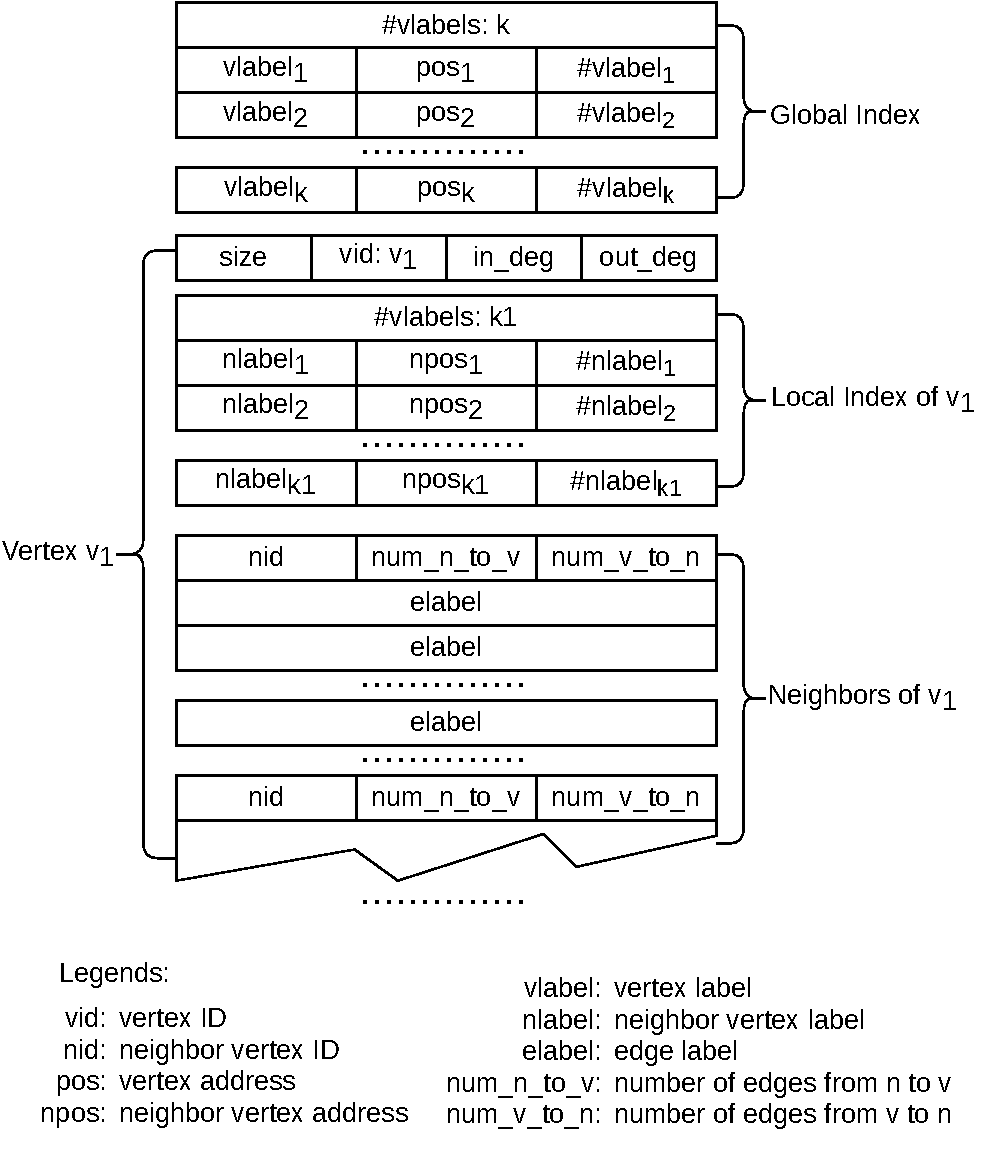
\includegraphics[width=0.48\textwidth]{img/data_graph.pdf}
  \caption{An I/O efficient property graph storage method that can boost the graph matching process.}\label{img:data_graph}
\end{figure}
